% ===================================================================
% Master's thesis. Estimating the Brent price effect of the 2026
% Strait of Hormuz disruption with a synthetic control ensemble.
% Compile:  pdflatex thesis  &&  bibtex thesis  &&  pdflatex thesis x2
% ===================================================================
\documentclass[11pt,a4paper]{article}

\usepackage[utf8]{inputenc}
\usepackage[T1]{fontenc}
\usepackage{lmodern}
\usepackage[margin=1in]{geometry}
\usepackage{amsmath,amssymb}
\usepackage{graphicx}
\usepackage{booktabs}
\usepackage{array}
\usepackage{multirow}
\usepackage{siunitx}
\usepackage{caption}
\usepackage{subcaption}
\usepackage{xcolor}
\usepackage{microtype}
\usepackage[round]{natbib}
\bibliographystyle{plainnat}
\usepackage[colorlinks=true,linkcolor=black,citecolor=blue!50!black,urlcolor=blue!50!black]{hyperref}

\setlength{\parskip}{0.35em}
\sisetup{detect-weight=true,detect-family=true}
\newcommand{\T}{\ensuremath{T_0}}

\title{\textbf{Pricing a Chokepoint:\\ A Synthetic-Control Estimate of the Brent Crude Premium\\ from the 2026 Strait of Hormuz Disruption}}
\author{Master Project, Data Science for Decision Making\\ Barcelona School of Economics}
\date{June 2026}

\begin{document}
\maketitle

\begin{abstract}
\noindent Roughly a fifth of the world's seaborne crude passes through the Strait of
Hormuz, so its disruption on 28 February 2026 was widely expected to move global oil
prices. Measuring that effect, however, is not straightforward: As Brent crude represents a unique global benchmark, there is no untreated control unit available from which a counterfactual price can be directly inferred. We construct that missing counterfactual with the \emph{synthetic control
method} (SCM), building a price path from a pool of 19 macro-financial donor series
(metals, agriculturals, equities, foreign exchange, rates, and volatility) chosen to share
Brent's exposure to common global factors while staying off the oil-supply causal path. To
keep the result from hinging on any single modelling choice, the synthetic is formed as the
median of an ensemble of five estimators with different inductive biases. We benchmark the framework using the Russian invasion of Ukraine on 24 February 2022, which represents the closest comparable historical oil supply shock. We then apply the framework to estimate the effects of a disruption in the Strait of Hormuz. Over the post-event window to
mid-June 2026 we find an average Brent premium of roughly \SI{56}{\percent} (ensemble
median; interquartile range \SIrange{51}{57}{\percent}), an estimate that is robust to placebo-based inference and a range of robustness and contamination checks. We frame the
estimate as a reduced-form, data-driven complement to the structural scenario estimates
produced by energy institutions, and discuss its use as an input to strategic-reserve,
monetary, and fiscal decisions.
\end{abstract}

\tableofcontents
\newpage
% ===================================================================
\section{Introduction}
\label{sec:intro}

The Strait of Hormuz is the narrowest binding constraint in the global oil system.
Roughly one-fifth of world petroleum-liquids consumption transits the lane between
Iran and Oman, carrying crude from Saudi Arabia, Iraq, the United Arab Emirates,
Kuwait, Iran, and Qatar to seaborne markets. What makes the chokepoint so
consequential is the absence of a redundant route. The Saudi East--West and UAE
Habshan--Fujairah pipelines together divert only a small fraction of this volume
overland, and no maritime bypass exists, so the overwhelming majority of Gulf crude
has nowhere else to go. This leaves Hormuz the single strongest bottleneck in the
world's oil-transport network. The lane has seen periodic near-misses, among them the
1980s tanker war, the 2019 Abqaiq strike, and recurring tensions through the mid-2020s,
each producing a transient risk-premium spike but never an actual closure. The
28~February 2026 disruption is the first realisation of that long-anticipated tail
risk.

Because crude oil is an input to almost every industry and a cost borne across nearly
all economies, a disruption on this scale was always going to move prices, and Brent
duly rose sharply in the days that followed. We study Brent rather than another
benchmark for two reasons. While the major crude indices are highly correlated and the
choice between them is largely immaterial, Brent is the reference price against which
the majority of internationally traded crude is settled, and we use its spot quotation
rather than a futures contract. Yet the raw price jump is uninformative on its own. It
conflates the disruption with everything else moving markets at the same time, and it
says nothing about how the effect evolves. This motivates a causal question:

\begin{quote}
\emph{What is the causal effect of the 2026 Strait of Hormuz disruption on the price
of Brent crude over a policy-relevant post-event window?}
\end{quote}

We deliberately target the \emph{total} causal effect rather than any single
transmission channel, and we estimate it as a \emph{path} over the post-event window
rather than a single number. The applications drive this choice. Emergency
strategic-reserve releases are sized against an implied price displacement. The
monetary-policy decision to look through an oil shock or to tighten turns on its size
and persistence. Fiscal stabilisation in subsidising oil importers scales with the
move. And sovereign hedging programmes price disruption scenarios against exactly such
magnitudes. Each lever acts on the trajectory of the effect, not on a peak-day figure.
The object we need is therefore the average gap between observed Brent and the price
that would have prevailed absent the disruption, traced over the whole window.
Recovering that counterfactual path, which has no directly observable analogue, is the
methodological core of this paper.

Standard observational designs cannot deliver it. Brent is a single, globally traded
benchmark, which rules out difference-in-differences (no panel of comparable treated
and control units), regression discontinuity (no running variable around a cutoff),
and instrumental variables (no credible instrument for a one-off geopolitical event).
The \emph{synthetic control method} \citep{abadie2010,abadie2021} is built for exactly
this situation. It forms a weighted basket of donor series whose pre-event co-movement
with the outcome is high and projects that basket forward as the counterfactual. It
yields a full counterfactual path rather than a point estimate, makes its identifying
assumptions auditable through the donor pool, and requires no structural stance on
whether the move is supply, risk premium, or expectations, since its estimand is a
reduced-form total effect.

The tools most commonly used to analyze such price shocks include event studies,
structural VARs, and institutional scenario models. However, they tend to address
narrower or different questions. Event studies measure abnormal returns in a short
window around the event but yield no multi-month path and miss persistence. Structural
VARs \citep{kilian2009,baumeisterhamilton2019} decompose prices into supply, demand,
and inventory shocks but produce no counterfactual path and rely on identification
restrictions with no settled precedent for a chokepoint event. And institutional
scenario models propagate an assumed barrel shortfall through a supply--demand model,
so their counterfactual is imposed rather than read from observed prices. We see these
as complements rather than competitors. Our cross-asset, data-driven estimate and a
structural scenario estimate answer different questions, the price gap implied by
observed co-movement versus the price implied by an assumed shortfall, so their
agreement is itself informative, and in practice the two can be used side by side.

Methodologically, our closest neighbour is the SCM-on-price design of
\citet{becker2021}. That work studies a regulated retail-fuel market with
cross-country donor units. Neither is available here, since Brent is a global crude
benchmark and no untreated country or market can serve as a donor. We therefore replace
geographic donors with cross-asset donors, including metals, agriculturals, equities,
foreign exchange, rates, and volatility, and apply the design under an exogenous
geopolitical treatment. To our knowledge this combination has not been used for any
previous oil shock, so the contribution is as much about establishing whether such a
design is valid in this setting as about the number it produces.

A single estimate, however, cannot be told apart from an artefact of the donor pool,
pre-window, model class, and regularisation. We therefore benchmark the design on the
nearest comparable historical oil-supply shock, the 2022 Russian invasion of Ukraine
(Brent \$95$\to$\$130 within two weeks), and check that the same machinery recovers
that documented magnitude before estimating the Hormuz effect afresh on its own
pre-window. We do not transfer the Russia fit to Hormuz. The two events sit in very
different market regimes, and we estimate each one independently. Because both are fit
on a common 19-series donor pool, we can additionally compare the donor weights across
regimes as a check on the stability of the factor structure SCM relies on.

To prevent any single modelling choice from driving the result, the synthetic is formed
as the median of an ensemble of five estimators with different inductive biases: convex
SCM, augmented SCM, elastic net, gradient-boosted trees, and Bayesian ridge. Fitting a
synthetic that tracks pre-event Brent closely is the easy part. The substantive work of
this paper is the validation that challenges the donor pool and the no-interference
assumption it rests on, namely placebo-based inference, leave-one-donor-out checks,
structural-break tests, a signed contamination-bias analysis, and a comparison against
na\"ive univariate counterfactuals. Our contribution is thus twofold: a data-driven
Brent-price ATT for the Hormuz disruption that complements existing structural
estimates, and a transparent template for validating cross-asset synthetic control
under a single-unit geopolitical treatment.

The remainder of the paper reviews the relevant literature (Section~\ref{sec:lit}),
sets out the factor model, estimand, and identifying assumptions
(Section~\ref{sec:theory}), describes the data and donor audit (Section~\ref{sec:data}),
details the empirical strategy and validation battery (Section~\ref{sec:methods}), and
reports results for both events (Section~\ref{sec:results}) before concluding
(Section~\ref{sec:conclusion}).


% ===================================================================
\section{Related Literature}\label{sec:lit}
% ===================================================================
We organise the review around problems rather than individual papers, because our
contribution sits at the intersection of three otherwise separate strands: how causal
counterfactuals are built for a single aggregate unit, how the oil-price effect of
geopolitical shocks is conventionally measured, and how inference is conducted with one
treated unit and a short post-period. Tools borrowed from machine learning and time
series are introduced where they are used (Section~\ref{sec:methods} and the
appendices). Here we position the causal design.

\subsection{Building counterfactuals for a single aggregate unit}
The problem of constructing a counterfactual for one treated unit is what synthetic
control was invented to solve. The method originates with \citet{abadiegardeazabal2003}
and \citet{abadie2010}, who build the counterfactual as a convex combination of
untreated donors matched on pre-treatment outcomes and formalise permutation (placebo)
inference for the single-unit case. \citet{abadie2015} extend it to comparative
politics, and \citet{abadie2021} codifies the practical requirements we adopt: a long,
shock-free pre-window, donors clean of the treatment (the SCM analogue of SUTVA), and a
good pre-treatment fit as a precondition for credibility. A subsequent literature
relaxes the convex-hull restriction. The augmented SCM of \citet{benmichael2021} adds a
ridge bias-correction permitting limited extrapolation when the treated unit lies
outside the donor hull, \citet{doudchenko2016} embed SCM, difference-in-differences, and
regression in a common regularised-regression family that allows unconstrained weights,
and \citet{athey2021mc} recast the problem as matrix completion. A caution runs through
all of it. Convex SCM weights are \emph{non-unique} when donors are correlated
\citep{abadielhour2021}, so many weight vectors yield near-identical fit and individual
weights should not be over-interpreted. We use this entire toolbox by running an
ensemble that spans the convex, augmented, and regularised-regression cases, and we read
cross-model weight dispersion through the non-uniqueness result rather than as
instability.

\subsection{Where SCM has been applied, and the gap we occupy}
Despite this methodological maturity, SCM has rarely been applied to a daily market
price. Most peer-reviewed applications estimate effects on \emph{non-price} aggregates
such as GDP, trade, and employment, including under discrete geopolitical shocks.
\citet{gharehgozli2017} estimates the GDP cost of sanctions on Iran and
\citet{mancini2024} the trade effect of the 2022 Russia--Ukraine war. The closest
mechanical precedent to a price application is \citet{becker2021}, who apply SCM to
Austrian retail fuel prices with other European countries as donors. That design differs
from ours in three ways that matter, as its treatment is an endogenous regulation rather
than an exogenous shock, its outcome an administered retail price rather than a traded
benchmark, and its donors cross-country rather than cross-asset. \citet{juarez2024} use
an oil-price shock as the treatment but on regional GDP, not on a price. The
intersection we occupy, which is SCM on a crude-benchmark \emph{price} under an exogenous
\emph{geopolitical} disruption with cross-asset donors, has no direct precedent, and
that is the gap this thesis addresses. Because the Hormuz event is recent, the only
existing analysis is institutional \citep{kiel2026,oies2026,worldbank2026,iea2026,
dallasfed2026}. These share one structure, namely to assume a barrels-per-day shortfall,
propagate it through a structural model, and output a price path, and none applies
synthetic control to the observed price. They form the comparison set against which we
position, and complement, our estimate.

\subsection{Oil prices and geopolitical risk: the incumbent methods}
The methods conventionally used for oil-price effects answer narrower or different
questions than ours. The dominant approach is the structural VAR with identified supply,
demand, and inventory shocks \citep{kilian2009,baumeisterhamilton2019}, with
\citet{hamilton2009} the narrative anchor for 2007--08. These decompose price changes
into structural components but yield no counterfactual path and require identification
restrictions for which a chokepoint event offers no standard precedent. A natural
alternative would regress oil prices on the Geopolitical Risk index of
\citet{caldara2022}, but this recovers the \emph{average} response to a unit of
geopolitical risk pooled across many events, a different object from the effect of one
specific disruption, and the index spikes endogenously to the very event we study, so it
can serve neither as our estimand nor as a clean donor. Short-window event studies
\citep{brownwarner1985} complete the incumbent set and give a magnitude but not the
multi-month path policy requires.

\subsection{Inference with one treated unit and a short post-period}
Our setting makes inference non-standard, and the recent literature counsels restraint
in two places. The first is inference itself. Permutation and placebo tests
\citep{abadie2010,abadie2015} are the field standard, with validity resting on an
approximate-symmetry assumption \citep{canay2017}. \citet{hahnshi2017} show that for
convex SCM this effectively requires Gaussian errors, which bounds how far placebo
$p$-values can be pushed for our nonlinear ensemble members, and \citet{chenyan2023}
formalise the in-time placebo into a mixed test with a permutation $p$-value. The second
is pretesting. \citet{roth2022} shows that pre-trend tests have low power at applied
sample sizes and can manufacture false confidence, and \citet{rambachanroth2023} propose
bounding rather than testing such violations, so we accordingly adopt a
report-and-interpret stance toward pre-period diagnostics rather than imposing pass/fail
thresholds. Finally, the value of a donor depends on how reliably it tracks the common
factor. A literature on matching reliability before differencing shows that a good
pre-period fit can \emph{mask} rather than remove contamination, the logic we use to
split donors by pre-window factor $R^2$ when signing the contamination bias
(Section~\ref{sec:results}). Multiple testing across donors is controlled by
Benjamini--Hochberg \citep{benjaminihochberg1995}.

% ===================================================================
\section{Conceptual Framework}\label{sec:theory}
% ===================================================================
This section sets out the data-generating process we assume for Brent, derives the
estimand and identifying assumptions from it, and explains why an \emph{ensemble} of
estimators is the appropriate proxy when the functional form of the counterfactual is
unknown. The factor model in Section~\ref{sec:theory}.1 is the organising device. It
makes donor selection an economic exercise, renders each identifying assumption
transparent, and gives the contamination bias an explicit sign.
\subsection{A factor model of Brent}
We decompose log Brent into a component spanned by global macro-financial factors common
to many assets and an oil-specific component:
\begin{equation}
p^{\text{Brent}}_t \;=\; \underbrace{\lambda' F_t}_{\text{common global factors}}
\;+\; \underbrace{o_t}_{\text{oil-specific (supply, chokepoint, geopolitics)}}
\;+\; \varepsilon_t .
\label{eq:factor}
\end{equation}
$F_t$ collects the five drivers that move Brent in normal times, namely the global
industrial cycle, the US dollar, real interest rates, global risk appetite, and China
demand, each proxied by non-oil assets. The oil-specific term $o_t$ is the object of
interest, the supply and chokepoint component a Hormuz disruption shifts. Each donor $j$
admits its own factor representation $X_{jt}=\gamma_j'F_t+u_{jt}$ with, by construction,
\emph{zero loading on} $o_t$. A clean donor is exposed to the same global factors as
Brent but is not physically routed through oil supply. A synthetic control is then a
weighted donor basket $\hat p_t=\sum_j w_j X_{jt}$, and the logic of the method follows
directly from \eqref{eq:factor}. If the weights reproduce Brent's factor loadings,
$\sum_j w_j\gamma_j\approx\lambda$, the basket tracks Brent through the pre-window, where
$o_t$ is small and stable. When a chokepoint shock fires, $o_t$ jumps for Brent but not
for the basket, the two decouple, and that decoupling \emph{is} the estimated premium.
Donor selection is therefore the economic exercise of spanning $F_t$ while excluding
$o_t$, that is, choosing identification over fit. This is precisely why the energy
complex (WTI, refined products, petrocurrencies), despite the highest raw correlation
with Brent, is excluded by design. It loads on the very $o_t$ we are trying to measure.
\subsection{Potential outcomes and the estimand}
Equation~\eqref{eq:factor} describes the observed price, while the causal question
concerns the price that would have prevailed without the event. Let $Y_t^N$ be Brent's
potential log-price absent the disruption and $Y_t^I$ under it, with treatment beginning
at \T{}. The treated-unit effect is $\tau_t=Y_t^I-Y_t^N$ for $t\ge$\T{}. With only one
treated unit, $Y_t^N$ is never observed after \T{}. The synthetic supplies the missing
term, $\hat Y_t^N=\sum_j w_j X_{jt}$, and the estimated effect is the gap
$\hat\tau_t=Y_t^I-\hat Y_t^N$, reported in percent as
$\text{gap}_t=100\,[\exp(Y_t^I-\hat Y_t^N)-1]$. We summarise the post-window by the
\emph{average treatment effect on the treated},
\begin{equation}
\widehat{\text{ATT}} \;=\; \frac{1}{|W|}\sum_{t\in[\T{},\,\T{}+W]} \text{gap}_t .
\end{equation}
We prefer the ATT to the peak or terminal gap for two reasons. It integrates over the
entire path, including any reversion, which is the object that reserve sizing, monetary
pass-through, and fiscal buffering act on, and averaging dampens single-day jumps from
liquidity or futures-roll mechanics.
\subsection{Identifying assumptions}
Because the synthetic stands in for an unobserved counterfactual, the estimate is only as
credible as the assumptions that license it, and the factor model makes each one
explicit and checkable.
\begin{enumerate}
\item \textbf{Common-factor spanning (pre-period fit).} The donor basket must reproduce
Brent's factor loadings, so that good pre-event tracking reflects shared $F_t$ rather
than coincidence. Checked by pre-period RMSPE, walk-forward cross-validation, and moment
matching.
\item \textbf{Donor cleanliness (SUTVA / no interference).} No donor may carry the
treatment. The loading $\gamma_j$ must not load on $o_t$, and donor $j$ must not be hit
through a channel specific to the focal event. Defended by an a-priori audit and
confirmed by model-agnostic break tests at \T{}.
\item \textbf{Regime stability.} The loadings $\lambda,\gamma_j$ must hold across the
pre-window and the projection window, so that a basket which tracked Brent before \T{}
remains a valid counterfactual after it. Checked by distance-correlation and
structural-break diagnostics, and, across events, by comparing donor weights between
regimes.
\end{enumerate}
Assumptions~1 and 3 are testable from observed data, whereas assumption~2 is the
genuinely untestable one, since donor cleanliness concerns the unobserved
$X_{jt}^N$. The next subsection shows how the factor model nonetheless lets us sign the
\emph{direction} in which a violation of assumption~2 would move the estimate.
\subsection{The direction of contamination bias}
The factor representation turns the informal worry that ``the donors might be affected by
the war'' into a quantity with a definite sign. Writing $\delta_{jt}=X_{jt}-X_{jt}^N$ for
the event-induced component of donor $j$, the estimation error is, as an exact identity,
\begin{equation}
\hat\tau_t-\tau_t \;=\; Y_t^N-\hat Y_t^N \;=\; -\sum_j w_j\,\delta_{jt}.
\label{eq:bias}
\end{equation}
The bias is \emph{minus} the weight-averaged donor contamination. Its sign is therefore
an empirical matter rather than an assumption. If contaminated donors are pushed
\emph{up} (oil-linked terms-of-trade, inflation$\to$rates), the synthetic is pulled up
and the ATT is \emph{under}-estimated, which is conservative. If they are pushed
\emph{down} (demand crowd-out, risk-off), the ATT is over-estimated. The identity
\eqref{eq:bias} is exact, but $\delta_{jt}$ is itself unobserved, so signing the bias in
practice requires estimating each $\delta_{jt}$ against a Brent-free reference, a
deliberately naïve construction whose assumptions and limits we set out, and apply, in
Section~\ref{sec:results}. What the theory delivers here is the \emph{structure}, which
is which way a given contamination pushes the estimate, not a certified magnitude. The
same identity also distinguishes two regimes of contamination by timing.
\emph{Contemporaneous} contamination occurs at \T{} and is screened by the audit and
break tests. \emph{Delayed} contamination accrues over the post-window, enters through
the projection, biases the gap toward zero, and grows with horizon, so a gap that
\emph{declines} as the window lengthens is its signature, and the short-horizon gap is
the least-contaminated estimate.
\subsection{Why an ensemble}
A single specification cannot be trusted because the counterfactual's functional form is
unknown. Equation~\eqref{eq:factor} need not be linear in the donors, and the
convex-hull restriction of classical SCM may or may not bind. Rather than commit to one
form, we proxy the counterfactual with five estimators whose inductive biases bracket the
plausible cases (Table~\ref{tab:models}): a simplex-constrained average, a
ridge-extrapolating correction, a sparse signed regression, a nonlinear tree ensemble,
and a Bayesian linear model. An estimated premium that survives across biases this
different is far more likely to reflect a real effect than a single-model artefact. We
report the cross-model \emph{median} as the headline, which is robust to any one model
misbehaving, and the inter-quartile range as a model-uncertainty band that complements
each model's own within-model interval.
\begin{table}[t]
\centering
\caption{The five-estimator ensemble. Each contributes a distinct inductive bias, and
the headline is the cross-model median gap.}
\label{tab:models}
\small
\begin{tabular}{@{}p{2.6cm}p{7.4cm}p{4.0cm}@{}}
\toprule
Estimator & Inductive bias & Reference \\
\midrule
Convex SCM & Non-negative donor weights summing to one, synthetic inside the donor convex hull & \citet{abadie2010}\\
Augmented SCM & Convex SCM plus ridge bias-correction, limited extrapolation outside the hull & \citet{benmichael2021}\\
Elastic net & Signed, sparse$+$ridge regression, lasso term drops donors entirely & \citet{doudchenko2016}\\
Gradient boosting (XGBoost) & Nonlinear, tree-based, captures interactions, cannot extrapolate beyond the training range & \citet{chenguestrin2016}\\
Bayesian ridge & Bayesian linear regression on donor levels (regression component of BSTS), conjugate Gaussian--Gamma prior & \citet{brodersen2015}\\
\bottomrule
\end{tabular}
\end{table}
A note on labelling: the fifth estimator is a Bayesian \emph{ridge} regression, not full
Bayesian structural time series. It implements only the regression-on-donors component
$\beta'x_t$ of \citet{brodersen2015} and omits the trend, seasonal, and spike-and-slab
selection components. At our sample size, and with no strong weekly seasonality, the
regression term carries most of the signal, but the model is best read as a
Bayesian-flavoured diversifier rather than a state-space causal-impact estimator
(Appendix~\ref{app:bsts}).

% ===================================================================
\section{Data}\label{sec:data}
% ===================================================================
This section describes the outcome series, the donor candidates and the per-event
cleanliness audit that selects among them, and the sample windows over which each event
is fit and projected. Two themes recur and both follow from the factor model of
Section~\ref{sec:theory}. Donor selection is an identification choice rather than a
fit-maximising one, and the length of the estimation window is itself a SUTVA
consideration, not merely a sample-size one.

\subsection{Outcome and sources}
The outcome is the daily \emph{Europe Brent Spot Price FOB} (EIA series RBRTEd), in
USD per barrel, downloaded directly from the U.S.\ Energy Information Administration
\citep{eia_brent}. The donor candidates are 32 macro-financial series from Yahoo
Finance (futures, ETFs, FX, rates, volatility), updated incrementally so the panel
keeps pace with new data. Table~\ref{tab:sources} summarises the sources. All are public
and redistributable, and the panel is rebuilt from source on each run so the analysis is
reproducible against the latest available data (here, through 15~June~2026 for Brent,
the binding constraint given the EIA's roughly one-week publication lag, and
23~June~2026 for the donors).

\begin{table}[h]
\centering
\caption{Data sources. All series are daily and publicly redistributable.}
\label{tab:sources}
\small
\begin{tabular}{@{}p{3.0cm}p{3.6cm}p{7.0cm}@{}}
\toprule
Object & Source & Contents \\
\midrule
Brent spot (outcome) & EIA, series RBRTEd & Europe Brent Spot FOB, USD/bbl, 1987--present\\
Donor candidates (32) & Yahoo Finance & Metals, agriculturals, equities, FX, rates, credit, volatility, crypto\\
\bottomrule
\end{tabular}
\end{table}

\subsection{The donor pool and the SUTVA audit}
Donor selection is central to identification (Section~\ref{sec:theory}). A series
qualifies only if it (i) co-moves with Brent through common global factors, (ii) is
\emph{not} physically routed through the disruption being attributed, (iii) is liquid
and daily-traded, and (iv) has sufficient pre-history. Criterion (ii) is the SUTVA
(no-interference) condition and is enforced by a per-event audit that classifies each
donor as Clean, Mild, or Heavy. For \textbf{Russia 2022}, 13 of 32 donors are flagged
through identifiable channels, namely Russia/Ukraine grain exports (Wheat, Corn),
palladium supply concentration, the EU energy-crisis pass-through to EUR and the dollar
basket, and a sanctions-evasion narrative for Bitcoin. For \textbf{Hormuz 2026}, only
Cotton is flagged (the indirect oil$\to$polyester substitution channel), and no donor is
physically routed through the Strait.

To make the two events directly comparable, we fit both on a single shared 19-donor
pool, formed by retaining only the donors rated Clean for Russia, the more demanding of
the two audits. This reduces the 32 candidates to 19, and because the Russia
strict-clean set is itself a subset of the Hormuz clean set, every member stays clean
for both events. Cotton, flagged Mild for Hormuz, is therefore excluded on the strength
of the Russia audit rather than retained, so its indirect channel never enters the
shared pool. One donor, VIX, is borderline. A full-history Bai--Perron test
\citep{baiperron1998} flags a single break in its relationship with Brent on 2022-01-07,
about 7 weeks before the invasion. We treat that as a loading-stability signal rather
than a SUTVA violation, because it does not reproduce when the test is run on the
analysis window alone, and a sensitivity check shows that keeping or dropping VIX moves
the ensemble premium by less than 1 percentage point. We therefore retain VIX, which
keeps the volatility factor represented. The energy complex (WTI, refined products,
petrocurrencies) is excluded by construction. It has the highest raw correlation with
Brent but loads on the very oil-specific shock we measure. Table~\ref{tab:donors} lists
the 19-donor pool by factor category.

\begin{table}[h]
\centering
\caption{The shared 19-donor pool, by factor category. The full 32-donor pool adds
Russia-contaminated series (e.g.\ Wheat, Corn, Palladium, EUR, DXY, BTC, Copper, Iron
Ore, US10Y) used only in the appendix robustness pool and as a contamination diagnostic.}
\label{tab:donors}
\small
\begin{tabular}{@{}lp{10.5cm}@{}}
\toprule
Category & Donors (shared pool) \\
\midrule
Metals (3) & Silver, Platinum, Gold \\
Agriculturals (3) & Coffee, Sugar, Live Cattle \\
Equities (2) & S\&P 500, Nikkei 225 \\
Foreign exchange (8) & AUD, JPY, CHF, CNY, INR, KRW, ZAR, MXN \\
Rates \& credit (2) & TLT (long Treasuries), HYG (high-yield credit) \\
Volatility (1) & VIX (implied S\&P 500 volatility) \\
\bottomrule
\end{tabular}
\end{table}

\subsection{Sample windows and summary statistics}
The estimation window must be chosen, not maximised. For daily-traded benchmarks like
Brent and its donors, a longer pre-history is not automatically better. These series
pass through distinct market regimes, and a window that spans several of them risks
teaching the synthetic a donor--Brent relationship that no longer holds in the
projection period, a regime shift that re-enters as post-event interference and thus as
a SUTVA violation. Our first task was therefore to locate the longest pre-window that
contains \emph{no} prior shock or regime break, rather than the longest pre-window
available. Each event then has such a pre-window (for fitting) and a post-window (for
projecting the counterfactual), each $\sim$20 months. Following \citet{abadie2021}, the
Russia pre-window starts 2020-07-01, deliberately \emph{after} the March--May 2020
cluster (OPEC+ collapse, WTI-negative, acute COVID) that would otherwise impose an
abnormal factor loading. The Russia post-window is truncated at 2022-09-30, the last
business day before OPEC+'s October 2022 supply cut, a Brent-specific policy shock that
would confound the invasion premium. The Hormuz post-window extends to the latest
available data (2026-06-15). Table~\ref{tab:summary} reports summary statistics, and
Figure~\ref{fig:timeline} plots the full Brent series with both events.

\begin{table}[h]
\centering
\caption{Summary statistics of Brent spot (USD/barrel) over each event sample.
Pre/post split at $T_0$. Russia: $T_0$=2022-02-24; Hormuz: $T_0$=2026-02-28.}
\label{tab:summary}
\small
\begin{tabular}{@{}llrrrrr@{}}
\toprule
Event & Segment & $n$ (days) & Mean & SD & Min & Max \\
\midrule
\multirow{3}{*}{Russia 2022}
 & Full sample & 572 & 75.95 & 24.76 & 36.33 & 133.18 \\
 & Pre-window  & 421 & 64.26 & 16.39 & 36.33 & 101.66 \\
 & Post-window & 151 & 108.54 & 11.37 & 82.55 & 133.18 \\
\addlinespace
\multirow{3}{*}{Hormuz 2026}
 & Full sample & 515 & 76.95 & 14.30 & 59.93 & 138.21 \\
 & Pre-window  & 443 & 72.08 & 6.58 & 59.93 & 88.66 \\
 & Post-window & 72  & 106.92 & 12.31 & 77.24 & 138.21 \\
\bottomrule
\end{tabular}
\end{table}

\begin{figure}[h]
\centering
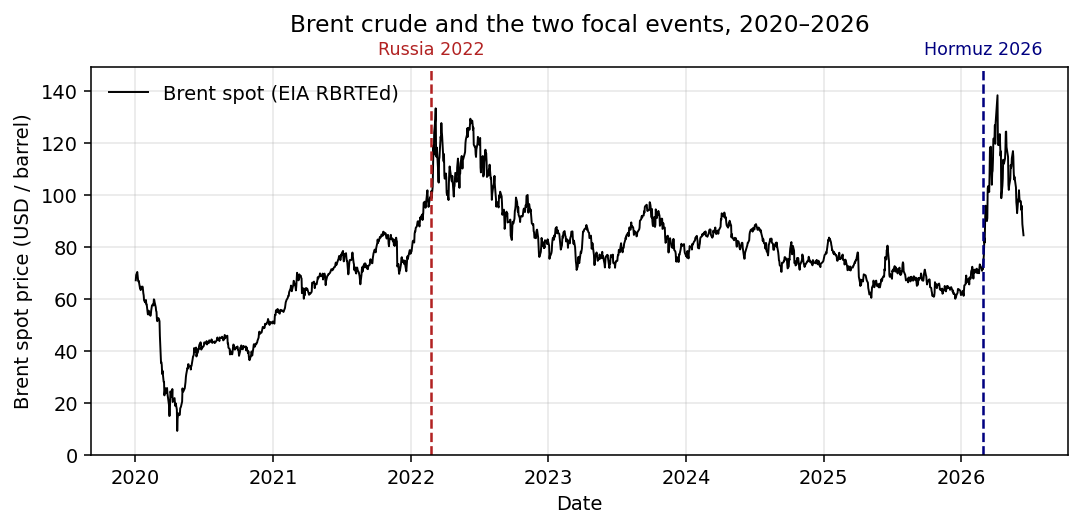
\includegraphics[width=0.92\textwidth]{figures/brent_timeline.png}
\caption{Brent crude spot price, 2020--2026, with the two focal event dates. Brent
roughly doubled after both shocks from a similar $\sim$\$75 base, but from very
different pre-event trajectories, a steep 2020--22 recovery rally before Russia and a
mild net decline through 2024--25 before Hormuz. This trajectory asymmetry is what makes
a na\"ive trend-extrapolation counterfactual unreliable (Section~\ref{sec:results}).}
\label{fig:timeline}
\end{figure}

The two pre-windows differ in a way that matters later. The Russia pre-period is
volatile (SD~\$16.4, spanning the COVID recovery and the 2021 reflation rally), while the
Hormuz pre-period is much calmer (SD~\$6.6). This difference drives much of the contrast
in the two events' inference, because a volatile pre-period widens the placebo
distribution and weakens Russia's permutation test even though its magnitude is
well-documented.


% ===================================================================
\section{Empirical Strategy and Validation}\label{sec:methods}
% ===================================================================
\subsection{Estimators}
All five estimators (Table~\ref{tab:models}) take the same input (log donor levels) and
target log Brent over the pre-window, then project the post-window counterfactual. The
two events are estimated entirely separately: they share the same 19-donor pool and the
same five-estimator pipeline, but each event trains its own models on its own pre-window,
so no parameter learned on one event is carried to the other. \emph{Convex SCM} solves
the classic nested optimisation: non-negative weights summing to one, chosen to minimise
pre-period RMSPE \citep{abadie2010}. \emph{Augmented SCM} adds a ridge penalty that
corrects for imperfect pre-fit and allows limited extrapolation \citep{benmichael2021}.
The \emph{elastic net} relaxes the simplex to signed, sparse coefficients
\citep{zouhastie2005,doudchenko2016}. \emph{XGBoost} fits shallow gradient-boosted trees
\citep{chenguestrin2016}, deliberately constrained (depth-2 stumps, strong
regularisation, row/column subsampling) for the small-sample regime. \emph{Bayesian
ridge} is a conjugate Bayesian linear regression on donor levels, the regression
component of BSTS \citep{brodersen2015}. Hyperparameters are tuned over small grids
(3--9 configurations) to bound the selection bias of \citet{cawley2010}; the convex SCM
has no tuned hyperparameter. Because the five estimators produce incommensurable weight vectors, a simplex for convex
SCM, signed unconstrained coefficients for the regressions, and no linear weights at all
for XGBoost, the ensemble operates on the \emph{gap series} each model implies rather
than on the weights. The headline at every $t$ is the cross-model median gap, with the
inter-quartile range as the model-uncertainty band.

\subsection{Validation battery and its logic}
A credible SCM estimate must clear three levels \citep{abadie2021}: pre-event fit, donor
identification, and inference. We organise the validation around these three levels and
run every test per model and per event.

The first level concerns \emph{fit}. Out-of-sample tracking is assessed by
expanding-window walk-forward cross-validation \citep{hyndman2018,bergmeir2012}. Its role
here is not model selection but evidence against over-fitting: a synthetic whose
out-of-sample pre-period tracking matches its in-sample tracking is reproducing a stable
donor--Brent relationship rather than memorising the pre-window, which is the empirical
content of the common-factor spanning assumption.

The second level concerns \emph{identification}, and is the donor-cleanliness battery
that defends the no-interference (SUTVA) assumption. Before any model is fit, each
donor's own return series is tested for a mean shift at $T_0$ using a permutation form of
the known-break test of \citet{chow1960} (rather than the unknown-break test of
\citet{andrews1993}, since the date is known), together with a Wilcoxon event-window test
\citep{brownwarner1985}; a donor is flagged if either rejects after Benjamini--Hochberg
FDR control \citep{benjaminihochberg1995}. Regime stability is checked with distance
correlation across pre-period thirds \citep{szekely2007} and with Bai--Perron break
dating \citep{baiperron1998,baiperron2003}, and an I(0)/I(1)-robust trend-break test
\citep{harvey2009,kpss1992} confirms that no donor's own trend breaks at either $T_0$;
the single VIX relationship-break noted in Section~\ref{sec:data} falls $\sim$7 weeks
\emph{before} the Russia $T_0$, not at it, and does not recur on the analysis window.
Empirically, for Hormuz 31 of 32 donors agree between audit and tests (only Cotton
differs); for Russia the tests confirm the broad picture and add one flag (CNY)
attributable to concurrent China dynamics rather than the war.

The third level concerns \emph{inference}. We run the in-space placebo, refitting each donor as a placebo treated unit and ranking
Brent's post/pre RMSPE ratio against the resulting distribution \citep{abadie2010} and
reading the permutation $p$-value with the symmetry caveat of \citet{hahnshi2017}. We add
the in-time placebo at a fake $T_0$ six months early, formalised as the mixed placebo test
of \citet{chenyan2023}, and a leave-one-donor-out check. Separately, as an exploratory
probe of regime stability rather than a validation test, we apply the weights fitted on
one event to the other event's window and read how far the pre-period fit degrades. We
report this transfer in Section~\ref{sec:results} for what it reveals about how regime-bound
the factor structure is, not as evidence for the headline magnitude, which rests entirely
on the separately fitted within-event ensemble.

% ===================================================================
\section{Results}\label{sec:results}
% ===================================================================
\subsection{Pre-event fit}
Table~\ref{tab:wfcv} reports walk-forward cross-validation. The pattern matches the two
events' pre-periods. For Hormuz, whose pre-period is calm, four of five models clear the
heuristic overfit flag and the fifth sits only just past it. For Russia, whose pre-period
spans the volatile 2020--22 recovery, more models trip the flag, because a noisy
pre-period inflates validation error. The flags do not exclude any model. They mark which
synthetics to read with more caution, and the most flagged model is also the one whose
headline gap is the ensemble outlier, so the flag and the outlier tell a consistent story.

\begin{table}[h]
\centering
\caption{Walk-forward cross-validation (5 expanding folds, 20-day horizons). A
validation/training RMSE ratio above 2 is a heuristic overfit flag, not an exclusion rule.}
\label{tab:wfcv}
\small
\begin{tabular}{@{}llrrl@{}}
\toprule
Event & Model & val/train RMSE & Flag \\
\midrule
Russia & Convex SCM     & 1.25 & OK \\
Russia & Augmented SCM  & 2.06 & overfit \\
Russia & Elastic net    & 1.99 & OK \\
Russia & XGBoost        & 3.24 & overfit \\
Russia & Bayesian ridge & 3.09 & overfit \\
\addlinespace
Hormuz & Convex SCM     & 1.40 & OK \\
Hormuz & Augmented SCM  & 1.54 & OK \\
Hormuz & Elastic net    & 1.51 & OK \\
Hormuz & XGBoost        & 1.84 & OK \\
Hormuz & Bayesian ridge & 2.28 & overfit \\
\bottomrule
\end{tabular}
\end{table}

\subsection{Headline estimates}
Table~\ref{tab:headline} reports the per-model post-window gap and the drift-adjusted gap
for both events, and Figure~\ref{fig:paths} plots the observed and synthetic paths. For
\textbf{Russia 2022} the ensemble-median premium is \SI{22.0}{\percent} over the
seven-month window (IQR \SIrange{10.9}{30.8}{\percent}), which implies a counterfactual
mean of \$88.6/bbl against an actual \$108.5. This is consistent with the documented
\$95$\to$\$130 move and its partial reversion by September. For \textbf{Hormuz 2026} the
ensemble-median premium is \SI{55.9}{\percent} over the window to mid-June (IQR
\SIrange{51.2}{56.6}{\percent}), with an actual post-window mean of \$106.9 against an
implied counterfactual near \$68.6. The Hormuz band is far tighter than Russia's, about
5 points against about 20, which reflects the calmer Hormuz pre-period.

\begin{table}[h]
\centering
\caption{Headline post-event gaps (\%). Drift-adjusted $=$ raw $-$ drift contribution.
Ensemble $=$ cross-model median, band $=$ IQR (Q25--Q75).}
\label{tab:headline}
\small
\begin{tabular}{@{}lrr@{\hskip 1.6em}rr@{}}
\toprule
& \multicolumn{2}{c}{Russia 2022 (7 mo)} & \multicolumn{2}{c}{Hormuz 2026 ($\sim$3.5 mo)}\\
\cmidrule(lr){2-3}\cmidrule(lr){4-5}
Model & Raw & Adj. & Raw & Adj. \\
\midrule
Convex SCM     & 33.6 & 28.4 & 55.9 & 57.3 \\
Augmented SCM  & 10.9 & 10.6 & 56.8 & 57.1 \\
Elastic net    & 22.0 & 21.2 & 56.6 & 57.4 \\
XGBoost        & 30.8 & 28.9 & 51.2 & 52.7 \\
Bayesian ridge & $-9.0$ & $-9.1$ & 43.0 & 43.0 \\
\midrule
\textbf{Ensemble median} & \textbf{22.0} & \textbf{21.2} & \textbf{55.9} & \textbf{57.1} \\
\textbf{IQR} & \textbf{[10.9, 30.8]} & n/a & \textbf{[51.2, 56.6]} & n/a \\
\bottomrule
\end{tabular}
\end{table}

\begin{figure}[h]
\centering
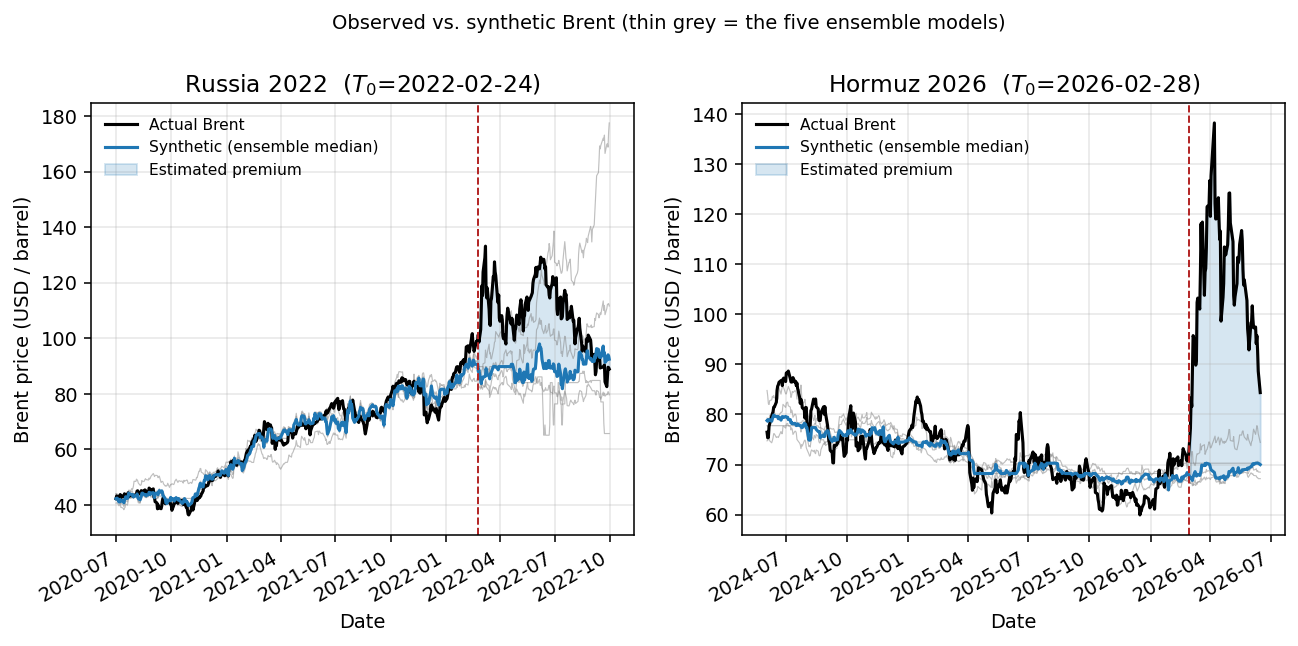
\includegraphics[width=\textwidth]{figures/counterfactual_paths.png}
\caption{Observed Brent (black) vs.\ the synthetic counterfactual. The thick blue line
is the ensemble-median synthetic, thin grey lines are the five individual models, and the
shaded region after $T_0$ (dashed red) is the estimated premium. The synthetics track
Brent closely before the event and decouple sharply afterward.}
\label{fig:paths}
\end{figure}

\paragraph{Economic reading of the model spread.} The cross-model dispersion has an
economic explanation rather than reflecting noise, and this is the one place where the
individual models matter, so we name them here. Convex SCM, confined to the simplex,
leans on the most stable donors, the FX block, as a trend baseline and adds
soft-commodity deltas such as Coffee and Sugar for Russia. The Bayesian ridge, with
unconstrained Gaussian coefficients, loads heavily and with large opposing signs on
currencies. For Russia those currencies moved with the simultaneous and historically
large Fed tightening cycle, a macro factor that has nothing to do with the invasion. That
confound is why the Bayesian ridge becomes the Russia outlier, with a negative full-window
gap, and why it carries the highest walk-forward flag. It is the expected behaviour of an
unregularised linear model in a pre-period that contains a strong non-event driver, and it
is the reason the ensemble uses the median rather than the mean. For Hormuz, whose calmer
pre-period has no analogous confound, the five models agree to within about 5 points.

\subsection{Inference: the in-space placebo}
Table~\ref{tab:placebo} and Figure~\ref{fig:placebo} report the in-space placebo. For
\textbf{Hormuz} the result is as strong as the test allows. Brent ranks first among all
placebo units under every model and both donor pools, with a post/pre RMSPE ratio between
6.9 and 10.2 that exceeds every donor's, so the permutation $p$-value sits at the
attainable floor, 0.050 in the 19-donor pool and 0.030 in the 32-donor pool. For
\textbf{Russia} no model reaches the floor, and XGBoost comes closest at $p=0.20$. The
reason is mechanical. The volatile 2020--22 pre-period gives the donors large pre-period
RMSPE as well, which widens the placebo distribution and lowers the test's power. This is a
known low-power property of the in-space placebo under a volatile pre-period
\citep{abadie2010}, not evidence of a small effect, and we validate Russia's magnitude
independently below.

\begin{table}[h]
\centering
\caption{In-space placebo permutation $p$-values and Brent's post/pre RMSPE ratio
(19-donor pool). Floor $=1/(N{+}1)$: 0.050 (19-donor), 0.030 (32-donor).}
\label{tab:placebo}
\small
\begin{tabular}{@{}llrrr@{}}
\toprule
Event & Model & $p$ (19-donor) & $p$ (32-donor) & Brent ratio \\
\midrule
Russia & best of five (XGBoost) & 0.20 & 0.15 & 7.75 \\
\addlinespace
Hormuz & Convex SCM     & \textbf{0.050} & \textbf{0.029} & 6.93 \\
Hormuz & Augmented SCM  & \textbf{0.050} & \textbf{0.029} & 8.45 \\
Hormuz & Elastic net    & \textbf{0.050} & \textbf{0.029} & 8.53 \\
Hormuz & XGBoost        & \textbf{0.050} & \textbf{0.029} & 10.19 \\
Hormuz & Bayesian ridge & \textbf{0.050} & \textbf{0.029} & 10.24 \\
\bottomrule
\end{tabular}
\end{table}

\begin{figure}[h]
\centering
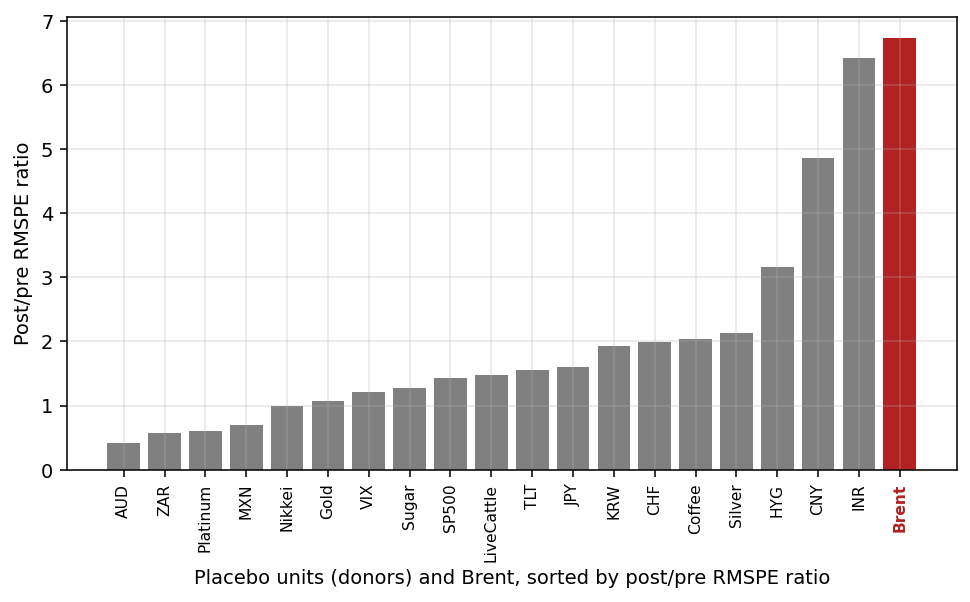
\includegraphics[width=0.72\textwidth]{figures/placebo_hormuz.png}
\caption{In-space placebo for Hormuz (convex SCM). Each bar is one unit's post/pre RMSPE
ratio. Brent (red) is the largest and ranks first among all 19 placebo units, so the
permutation test rejects at the attainable floor.}
\label{fig:placebo}
\end{figure}

\subsection{Robustness}
\paragraph{Russia magnitude and external validation.} Because Russia is a known event, we
validate its magnitude against the EIA's last two pre-invasion Short-Term Energy Outlook
forecasts, issued before 24 February 2022. These forecasts are an independent structural
counterfactual that shares no information path with the SCM. Over the identical 151-day
window the ensemble-median synthetic mean of \$88.6 sits within \$3.6 of the STEO
February 2022 forecast of \$84.9, and three of five models bracket the STEO anchor to
within \$4. Two independent methods landing on nearly the same counterfactual is strong
evidence that the SCM does not produce an implausible path.

\paragraph{Post-window horizon sensitivity.} Figure~\ref{fig:sensitivity} reports the gap
at 1, 2, 3, and 6-month and full horizons. The two events show opposite and diagnostic
profiles. Russia declines with horizon, from about 31\% to 22\%, which is the signature of
delayed contamination as second-round war channels switch on through 2022 and pull the
synthetic up. The full-window figure is therefore conservative, and the
least-contaminated one-month estimate is about 31\%. Hormuz rises and then eases, from
about 46\% to 59\% and back to 56\%, which is the opposite of attenuation. The chokepoint
premium builds in and holds, and the slight easing at the full horizon reflects Brent's
partial mid-June pullback that appears once we extend the window to the latest data. The
same diagnostic declining for Russia and rising for Hormuz shows that it is not a
mechanical artefact.

\begin{figure}[h]
\centering

\includegraphics[width=0.78\textwidth]{figures/postwindow_sensitivity.png}
\caption{Ensemble-median gap by post-event horizon (shaded $=$ IQR across models). Russia
attenuates with horizon, the delayed-contamination signature, while Hormuz rises and then
plateaus as the premium builds in and holds.}
\label{fig:sensitivity}
\end{figure}

\paragraph{Leave-one-donor-out.} Dropping each weighted donor in turn leaves the focal
Hormuz estimate tight around its baseline across all models (convex 51.2 to 59.3, ASCM
54.6 to 60.5, elastic 55.2 to 62.2, XGBoost 51.6 to 57.7\%), so no single donor drives the
result. For Russia we report the ensemble-median range rather than every model, because
Russia's wider spread comes from the simplex models' reliance on a few soft-commodity
donors, the same concentration that drives the contamination finding below. Read that way,
the wider Russia range (for example convex 32.8 to 59.6\%) is itself a symptom of the
donor-quality issue rather than a separate concern.

\paragraph{Cross-event weight stability.} As an exploratory probe rather than a validation
test, we apply the weights fitted on one event to the other event's window and read how far
the pre-period fit degrades. The transfer is weak, and that weakness is informative. Only
convex SCM transfers to a clearly positive Hormuz premium, at 25.3\% with a degraded but
non-pathological pre-fit, while the other models move toward or below zero with pre-fit
errors many times their independent level (Table~\ref{tab:transfer}). The reason is that
the two pre-periods are different factor regimes. Russia's 2020--22 pre-period is shaped by
the COVID recovery and the onset of Fed tightening, whereas Hormuz's 2024--26 pre-period is
a calmer disinflation regime, so the donor-to-Brent loadings that the weights encode do not
carry across. The models that fail hardest are the ones that load most on currencies, and
the dollar and emerging-market FX relationships shifted most between the two regimes.
Extending the Hormuz window through the June pullback widens the regime gap further. We
therefore read the transfer as weak and convex-only corroboration that some positive
premium survives a change of regime, and as direct evidence that fitting each event
separately is the correct choice, not as confirmation of the level.

\begin{table}[h]
\centering
\caption{Cross-event weight stability probe: Russia-fitted weights applied to Hormuz.
Independent and transferred pre-period RMSPE in log units.}
\label{tab:transfer}
\small
\begin{tabular}{@{}lrrrr@{}}
\toprule
Model & Indep.\ gap (\%) & Transf.\ gap (\%) & Indep.\ RMSPE & Transf.\ RMSPE \\
\midrule
Convex SCM     & 55.9 & 25.3   & 0.066 & 0.336 \\
Augmented SCM  & 56.8 & $-0.8$  & 0.066 & 0.467 \\
Elastic net    & 56.6 & $-68.6$ & 0.054 & 1.513 \\
XGBoost        & 51.2 & $-44.1$ & 0.053 & 0.928 \\
Bayesian ridge & 43.0 & $-100.0$ & 0.037 & 18.567 \\
\bottomrule
\end{tabular}
\end{table}

\paragraph{Na\"ive counterfactual floor.} We compare the SCM against donor-free univariate
counterfactuals built only from Brent's own past (Table~\ref{tab:naive}), and the
comparison yields three findings. First, the SCM adds value. It sits about 13 points above
the trend-free random-walk null for Russia and about 7 points above it for Hormuz, so the
donor machinery extracts something that extrapolating Brent's own series cannot. Second,
and most telling, the naive bias flips sign across the two events purely because the
pre-window trend sign differs. The linear trend extrapolates Russia's recovery rally upward
and returns an implausible negative full-window gap of about $-4\%$, yet the same method
extrapolates Hormuz's mild downtrend and inflates the gap to about 71\%. A counterfactual
built from one series alone is therefore regime-fragile in a way the donor-based SCM is not.
Third, for Russia the SCM and the trend extrapolation sit on opposite sides of the truth.
The SCM leans high, as the contamination analysis below confirms, and the trend
extrapolation leans low, so the two bracket the real value, with the random-walk null at
$+8.7\%$ the most defensible naive point. The naive floor and the contamination analysis
thus corroborate each other, one from a donor-free direction and one from a donor-based one.

\begin{table}[h]
\centering
\caption{SCM vs.\ na\"ive univariate counterfactuals, full-window gap (\%). RW flat and
RW drift are the random-walk carry and the drifted random walk, Lin.\ trend is the linear
pre-trend extrapolation, and ARIMA is the AIC-selected model, which reduces to a driftless
random walk for both events.}
\label{tab:naive}
\small
\begin{tabular}{@{}lrrrr@{}}
\toprule
Event & SCM median & RW flat & RW drift & Lin.\ trend \\
\midrule
Russia & 22.0 & 8.7  & $-6.9$ & $-4.2$ \\
Hormuz & 55.9 & 48.9 & 49.8   & 70.9   \\
\bottomrule
\end{tabular}
\end{table}

\paragraph{Sign of the contamination bias.} This last check is a deliberately naive and
directional diagnostic, not a structural correction. It does not prove that the donors are
clean. It asks a narrower question. If some contamination remains despite the audit and the
break tests, which way would it bias the estimate? We answer it with equation~\eqref{eq:bias}
and a Brent-free reference, and the two events give opposite and informative answers. For
\textbf{Hormuz}, where every other check already supports a stable estimate, any residual
contamination has a small negative sign, between about $-1$ and $-8\%$. The reading is
reassuring in one direction. If the estimate is biased at all, it is biased downward, so the
true premium is at least as large as we report and the headline is conservative. For
\textbf{Russia} the sign reverses and the bias is large and positive, on the order of
$+13$ to $+21\%$. The reason is economic. The high-price and risk-off environment of 2022
depressed the demand-cyclical donors, the equities, metals, and soft commodities, relative
to the safe-haven and currency donors, so the synthetic built from them sits too low and the
gap reads too high. The bias concentrates in the low-reliability soft-commodity donors, and
splitting donors by pre-window factor $R^2$ confirms that most of it sits in the
low-reliability group rather than in the donors that track the common factor well. The
conclusion is asymmetric. Contamination is conservative for the focal Hormuz estimate and
inflates the Russia full-window number, so Russia's magnitude validation rests on the early
and peak window, where the \$95$\to$\$130 move is recovered, and not on the attenuated
full-window average.

\subsection{Interpretation}
The 2026 Hormuz chokepoint premium is roughly \SI{56}{\percent} of Brent's no-event level
over the first three and a half months, and the estimate is stable. It holds across all
five estimators and clears the validation battery of Section~\ref{sec:methods}, with the
in-space placebo reaching its attainable floor as the strongest single result. The
contamination analysis adds a useful direction to this stability. If anything, the true
Hormuz premium is larger than our estimate, not smaller. The cross-event probe is the
weakest of the checks, and we lean on it only for the sign of the effect under a change of
regime, never for its level. We read the estimate as a complement to the structural
scenario estimates from energy institutions rather than a competitor to them. Those answer
the question of what price an assumed barrel shortfall implies, while the SCM answers what
price gap the observed cross-asset co-movement implies, and the two questions inform
different parts of a policy response. For the levers set out in Section~\ref{sec:intro},
reserve releases, monetary pass-through, and fiscal buffers, the relevant input is the
integrated path-level premium, and the estimate here supplies it together with an auditable
identification argument.

\subsection{Limitations}
Four limitations bound what we can claim. First, the design has a single treated unit and a
short post-period, which caps the power of permutation inference. The Hormuz placebo reaches
0.050, which is the best value attainable at this sample size rather than a conventional
rejection, so we read it as the strongest available signal and not as a small p-value in the
usual sense. Second, the estimand is a reduced-form total effect. It captures the full price
gap but does not separate the premium into a physical-supply component, a risk-premium
component, and an expectations component, which some policy uses would want to distinguish.
Third, the Hormuz event is recent and has no documented post-event counterfactual of its own,
so its validation is internal and rests on the Russia case as a calibration by analogy rather
than on an external ground truth. Fourth, the factor structure is regime-bound, as the weak
cross-event transfer shows directly. The estimate is valid for the regime of this event and
should not be read as a general chokepoint premium that would recur unchanged in a different
macro environment. Underlying all four is that donor cleanliness is only partly testable. The
no-interference assumption concerns an unobserved counterfactual donor path, and the
contamination-sign diagnostic is naive and directional, so it bounds the likely direction of
any residual bias without proving that none exists.

% ===================================================================
\section{Conclusion}\label{sec:conclusion}
% ===================================================================
We estimated the Brent-price effect of the 2026 Strait of Hormuz disruption by building a
counterfactual with an ensemble synthetic control and benchmarking the design against the
documented Russia 2022 shock. Over the window to mid-June 2026 the ensemble-median premium
is roughly \SI{56}{\percent} of Brent's no-event level (IQR 51 to 57\%), large and positive
under every estimator. The estimate clears the validation battery. Brent ranks first among
all units in the in-space placebo at the attainable floor, the leave-one-out check stays
tight, the contamination-bias sign points conservative, and the synthetic beats the naive
univariate baselines. On the benchmark event the same machinery recovers a magnitude
consistent with the documented \$95 to \$130 move and within \$3.6 of the EIA's pre-invasion
structural forecast, which gives independent reassurance that the method tracks a real path.

The contribution is twofold. The substantive result is a data-driven Brent premium for the
Hormuz disruption that complements the structural scenario estimates produced by energy
institutions. The methodological result is a transparent template for validating cross-asset
synthetic control under a single-unit geopolitical treatment, with an identification argument
a reader can audit donor by donor. Our approach and the structural one answer different
questions. The structural models ask what price an assumed barrel shortfall implies, while
the synthetic control asks what price gap the observed co-movement of global markets implies.
Because the two read the event from different directions, they work best together, and our
estimate is a complement to scenario analysis rather than a substitute for it.

For policy the relevant object is the integrated, path-level premium rather than a single
peak-day figure, and that is what the estimate supplies. Reserve sizing, the monetary
decision to look through or tighten, fiscal buffering in oil importers, and sovereign hedging
all act on the magnitude and persistence of the price move, and a counterfactual path lets a
decision maker read both at once and update as new data arrive.

Several limitations bound the estimate. The design has a single treated unit and a short
post-window, so the inference tests are under-powered and the placebo can only reach its
floor. The estimand is a reduced-form total effect and does not separate supply, risk, and
expectations. The Hormuz event is recent and has no external counterfactual of its own, so
its validation is internal and leans on the Russia benchmark by analogy. The factor structure
is regime-bound, as the weak cross-event transfer shows. None of these overturns the central
finding. The observed co-movement of global markets with Brent implies that the 2026 Hormuz
disruption added a large and robust premium to crude, on the order of half its no-event price,
and the estimate is meaningful and usable for the decisions that depend on it.


\bibliography{references}

\appendix
% ===================================================================
\section{Robustness grid}\label{app:grid}
% ===================================================================
The headline uses the preferred specification (shared 19-donor pool, preferred pre-window,
ensemble median). The full grid varies (i) the pre-window (preferred, extended, and narrow
specifications); (ii) the donor pool (shared 19, permissive 26 for Russia, full 32); and
(iii) the model (each of the five plus the median). For Russia the donor-pool sweep is
itself a diagnostic: the gap is expected to \emph{shrink} monotonically from the clean
19-donor pool to the contaminated 32-donor pool, because Russia-treated donors get inflated
by the same shock and pull the synthetic up. If this monotonic pattern holds, the
SUTVA-driven exclusion logic is empirically supported.

% ===================================================================
\section{Bayesian ridge and full BSTS}\label{app:bsts}
% ===================================================================
The fifth ensemble member implements only the regression-on-donors term $\beta'x_t$ of the
Bayesian structural time-series model of \citet{brodersen2015}, with a conjugate
Gaussian--Gamma prior. It omits the local-linear \emph{trend}, the \emph{seasonal}
component, the \emph{spike-and-slab} donor selection, and the autocorrelation-aware
posterior over the full state trajectory. At our sample size, with no strong weekly
seasonality in daily oil prices, the regression term carries most of the signal, so the
proxy is an adequate Bayesian-flavoured diversifier; but its credible intervals are Gaussian
and ignore autocorrelation, and its donor ``importances'' are standardised-coefficient
magnitudes, not true posterior inclusion probabilities. We therefore call it a Bayesian
ridge regression rather than a BSTS, and read its placebo $p$-values as rank statistics
rather than formal probabilities (Table~\ref{tab:placebo}). A full BSTS implementation is the
natural route to autocorrelation-aware credible intervals in a future iteration.

% ===================================================================
\section{Structural-break tests}\label{app:breaks}
% ===================================================================
Two break tests support donor screening. \emph{Bai--Perron}
\citep{baiperron1998,baiperron2003} dates breaks in the donor--Brent weekly-return
relationship $r^{\text{donor}}_t=\alpha_s+\beta_s r^{\text{Brent}}_t+\varepsilon_t$ by
globally minimising segment SSR via dynamic programming, with the break count chosen by BIC.
Only VIX shows a break strictly inside a pre-window (2022-01-07). We treat the break tests as
informative rather than automatically disqualifying: the VIX break is a loading-stability
signal, it does not reproduce on the analysis window alone, and the in/out sensitivity is
below 1 pp, so VIX is retained (Section~\ref{sec:data}). The relationship specification is
Brent-based, so a break \emph{at} $T_0$ is ambiguous; the
complementary \citet{harvey2009} trend-break test resolves this by testing the donor's
\emph{own} log-level trend with a statistic whose asymptotic size is invariant to whether the
series is I(0) or I(1): it weights an I(0)-optimal and an I(1)-optimal sup-$t$ statistic by
KPSS stationarity weights \citep{kpss1992}. Empirically all 32 donors are classified I(1)-like
and none rejects a trend break within $\pm$8 weeks of either $T_0$, so no retained donor was
itself trend-treated by either event.

\end{document}
